\chapter{Locomotion}
\section{Fortbewegungsarten}
\begin{itemize}
	\item Fortbewegungsarten für Roboter sind of durch die Natur inspiriert.
	\item Roboter mit Beinen benötigen in der Regel mehr Freiheitsgrade und sind mechanisch komplexer als Roboter auf Rädern.
\end{itemize}
\section{Laufroboter}
\subsection{Vorteile von Laufrobotern}
\begin{itemize}
	\item Können auf unregelmäßigen Untergrund laufen
	\item Natürliche Fortbewegung
	\item Keine Umweltveränderung erforderlich
\end{itemize}
\subsection{Nachteile von Laufrobotern}
\begin{itemize}
	\item Komplizierte Mechanik
	\item Anspruchsvolle Steuerungssoftware
	\item Mehrere Freiheitsgrade pro Beins
	\item Vielzahl an Sensoren erforderlich
	\subitem interne Sensoren wie Potentiometer, Inkrementalsensoren, ...
	\subitem externe Sensoren wie Stoßdämpfer, Stereo-Kamera, Infrarot, Ultraschall, ...
\end{itemize}
\subsection{Freiheitsgrade für Roboterbeine}
\begin{itemize}
	\item Um ein Bein bewegen zu können, sind mindestens zwei Freiheitsgrade notwendig
	\item Die meisten Laufroboter haben mehrgliedrige Beine mit mindestens drei Freiheitsgraden pro Bein
\end{itemize}
\begin{figure}[H]
	\begin{center}
		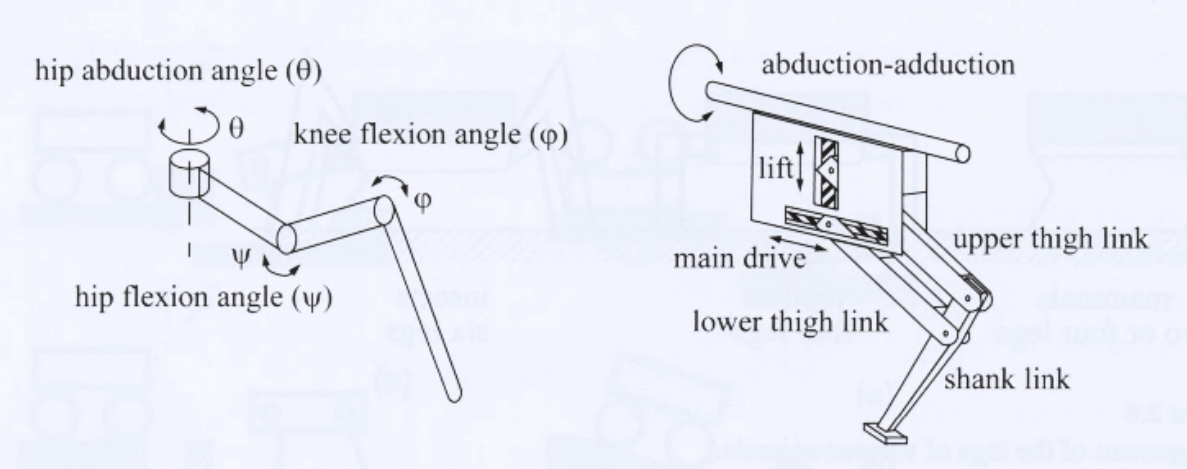
\includegraphics[scale=0.5]{Resources/PNG/RoboterFreiheitsgrade.PNG}
		\caption{Freiheitsgrade für Roboterbeine}
		\label{fig:Resources/PNG/RoboterFreiheitsgrade.PNG}
	\end{center}
\end{figure}
\subsection{Freiheitsgrade für Zweibeiner}
\begin{itemize}
	\item Zweibeiner haben meist sechs Freiheitsgrade pro Bein
	\item Menschliches Bein hat 7 Freiheitsgrade
	\item Die Zahl der unterschiedlichen Gangarten hängt von der Zahl der Beine ab.
	\item Ein Zweibeiner (mit $k=2$) hat $N = (2 \cdot k - 1)! = 6$s unterschiedliche Gangarten
\end{itemize}
\subsection{Laufverhalten}
\begin{itemize}
	\item Das Geh- und Laufverhalten kann in \textbf{statisch und dynamisch stabile Gangarten} eingeteilt werden 
	\item Funktioniert nur für sehr langsame Bewegungen
\end{itemize}
\paragraph{Definition: Statisches stabiles Gehen}
bedeutet, dass sich der Roboter zu jedem Zeitpunkt in einem statischen Körperschwerpunkt ist so über den Füßen, dass der Körper nicht fallen kann.
\paragraph{Definition: Dynamisch stabiles Gehen}
bezeichnet Laufbewegungen, mit weniger als drei Füßen in Kontakt mit dem Boden.
Dynamisches Gehen arbeitet mit Körperschwingungen: der Körperschwerpunkt befindet sich die meiste Zeit außerhalb von der aufgespannten Gleichgewichtszone.
\subsection{Statisch stabiles Gehen}
\begin{itemize}
	\item Statische Stabilitätsbedingung: der Masseschwerpunkt (\textit{Center of Gravity}) ist immer über dem STützpolygon
	\subitem \textbf{Stützpolygon} ist ein minimales Polygon, das alle Kontaktstellen des Roboters mit dem Boden enthält.
	\subitem möglich für alle Beinanzahlen >= zwei
	\subitem nur langsame Bewegungen möglich	
\end{itemize}
\paragraph{Dreifußgang}
\begin{itemize}
	\item Je drei Beine sind in der Stemmphase und in der Schwingphase
	\item Verbindet man die drei Beine in der Stemmphase ergibt sich ein Dreieck
\end{itemize}
\begin{figure}[H]
	\begin{center}
		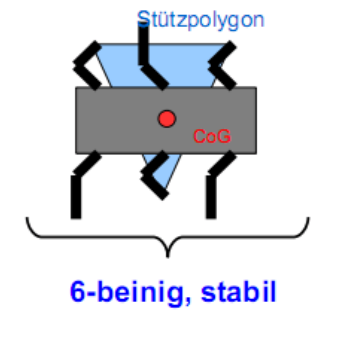
\includegraphics[scale=0.6]{Resources/PNG/DreiBein.PNG}
		\caption{}
		\label{fig:Resources/PNG/DreiBein.PNG}
	\end{center}
\end{figure}
\subsection{Zero Moment Point und Pseudo-Dynamisches Gehen}
\begin{itemize}
	\item Zero Moment Point (ZMP) ist der Punkt auf dem Boden, an dem die Kippmomente null werden
	\item ZMP dominiert seit 40 Jahren das zweibeinige GEhen
	\item Bewährt bei glatten Flächen
	\item Bei zweibeinigen Robotern wird das Stützpolygon ersetzt durch die konvexe Hülle der Bodenkontaktflächen
	\item \textbf{Nachteile des ZMP}
	\subitem ZMP geregelter Gang kann nicht schneller sein als die Sensorik
	\subitem ZMP erfordert die genaue Kenntnis der Massenverteilung im Roboter und alle Gelenkstellungen
\end{itemize}
\subsection{Steuerungssoftware}
\paragraph{Neuronale Netze}
\begin{itemize}
	\item Ähnlich zu biologischen Vorbildern
	\item Training durch Simulation
\end{itemize}
\paragraph{Mechatronik und Regelung}
\begin{itemize}
	\item Regelung von Gelenkwinkel und -Geschwindigkeiten
	\item Trajektorienplanung und -interpolation
	\item Explizite regelbasierte Laufplanung
	\item \textbf{Vorteil:} Nutzung gut bekannter mechatronischer Prinzipien 	
	\item Eigenschaften wie Stabilität sind gut bekannt
	\item Lernen einfacher Steuerungszusammenhänge im Gegensatz zu Neuronalen Netzen nicht notwendig
\end{itemize}
\paragraph{Verhaltensbasierte Steuerungen}
\begin{itemize}
	\item Modellierung von Basisverhalten durch Aufbau von Sensor/Motor-Verbindungen
	\item Zerlegung von komplexem Verhalten zu einer Vielzahl einfacher Ebenen mit zunehmend abstraktem Verhalten
	\item Verhalten können durch ein überlagertes Verhalten beeinflusst werden
	\item Mehrere Basisverhalten können zusammen zu einem völlig neuartigem Verhalten führen
	\item \textbf{Jedoch:} Schwierigkeiten bei der Realisierung komplexer Verhalten.
\end{itemize}
\section{Radroboter}
\subsection{Stabilität von Radrobotern}
\begin{itemize}
	\item Natürliche Bewegungen wie Kriechen, Laufen, Springen oder Gehen technisch schwer zu imitieren.
	\item Mehrheit der mobilen Roboter auf Rädern oder Raupen unterwegs
	\item Alle Räder haben in der Regel Kontakt zum Untergrund
	\item für \textbf{statisch stabile Fahrzeuge} braucht man mindestens drei Räder:
	\subitem Zwei angetriebene Räder auf einer Achse mit einem oder zwei passiv mitlaufenden Stützrädern, die sich frei drehen können
	\subitem Steuerung erfolgt durch verschiedene Geschwindigkeit angetriebener Räder
	\subitem kinematisches Zentrum oft in der Mitte des Fahrzeugs
	\item \textbf{dynamische Stabilität erfordert Bewegung}
\end{itemize}
\section{Kinematik mobiler Radroboter}
\subsection{Holonomische Bewegung}
Eine Bewegung heißt \textbf{holonomisch}, wenn das Objekt seine \textbf{Orientierung und seine Position unabhängig voneinander ändern} kann.
\paragraph{Pose System}
\begin{itemize}
	\item Position eines Objekts auf einer Ebene kann mittels zweier Koordinaten angegeben werden
	\item Die absolute Orientierung des Objektes wird mit einer dritten Koordinate angegeben, was zusammen ein Pose-System ergibt
	\item Koordinaten des Pose Systems $\Rightarrow$ 2 für die Position in x,y Ebene; 1 für die absolute Orientierung
\end{itemize}
\subsection{Kinematik und Positionsveränderung für Zweiradandtrieb}
\begin{itemize}
	\item \textbf{Vorraussetung}: kreisförmiger Roboter mit Zweiradantrieb, Bewegung ist nur in der Ebene möglich
	\item Position: Koordinaten $x,y$, Orientierung $\alpha$
	\item Roboter misst zu diskreten Zeitpunkten $t$ den mit dem linken bzw. mit dem rechten Rad zurückgelegten Weg
	\item $\Delta L$ und $\Delta R$ werden von Radwegsensoren ermittelt
\end{itemize}
\begin{itemize}
	\item Der Drehwinkel $\Delta \alpha$ ist die Wegdifferenz des rechten und des linken Rades geteilt durch den Radabstand $D$ \\
	$\Delta \alpha=\frac{\Delta R-\Delta L}{D}$
	\item Die Wegstrecke ist der mittlere Weg \\
	$\Delta s=\frac{\Delta L+\Delta R}{2}$
	\item Positionsänderung bei Geradeausfahrt mit $\Delta L = \Delta R$ \\
	$\Delta x=\Delta R * \cos (\alpha)$ \\
	$\Delta y=\Delta L * \sin (\alpha)$
\end{itemize}
\subsection{Fortbewegung bei Omnidirektionalem Antrieb}
\begin{figure}[H]
	\begin{center}
		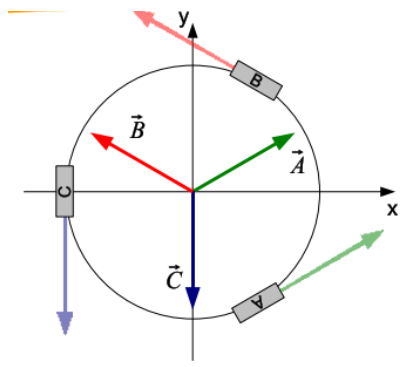
\includegraphics[scale=0.6]{Resources/PNG/EinheitsVektoren.PNG}
		\caption{Einheitsvektoren}
		\label{fig:PNG/EinheitsVektoren.PNG}
	\end{center}
\end{figure}
\begin{itemize}
	\item \textbf{Einheitsvektoren} geben die Richtungen an, in denen die Omniwheels von den drei Motoren angetrieben werden.
	\item \textbf{Geschwindigkeitsvektoren} sind die Einheitsvektoren
	\item Raddrehmomente $\alpha, \beta, \gamma$ proportional zur Winkelgeschwindigkeit des jeweiligen Rades
	\item \textbf{Bewegungsvektor} $\vec{V}=\alpha \cdot \vec{A}+\beta \cdot \vec{B}+\gamma \cdot \vec{C}$
\end{itemize}












	








